\documentclass[conference]{IEEEtran}

\usepackage[T1]{fontenc}
\usepackage{cite}
\usepackage{amsmath,amssymb}
\usepackage{graphicx}
\usepackage{booktabs}
\usepackage{array}
\usepackage{url}
\usepackage{xcolor}

\graphicspath{{figures/}}

\title{Medical Ultrasound Image Analysis: Acquisition, Segmentation, Classification, and Foundation Model Evaluation}

\author{
\IEEEauthorblockN{P0 Group: Student Name 1, Student Name 2, Student Name 3}
\IEEEauthorblockA{BME1307 Spring 2026\\
School of Biomedical Engineering\\
Email: \{student1, student2, student3\}@example.com}
}

\begin{document}

\maketitle

\begin{abstract}
This course project studies a complete medical ultrasound image analysis workflow, covering real ultrasound acquisition, carotid artery segmentation and quantification, breast ultrasound lesion classification, and foundation-model evaluation. For Part 1, eight neck ultrasound acquisitions were processed with a classical Hough-circle, wall-contrast, and Chan--Vese segmentation pipeline. The estimated carotid diameters were all within the literature range of 4.3--7.7 mm. For Part 2, 120 breast ultrasound samples were segmented using full-image, classical computer vision, refined Chan--Vese, and BUSAT masks, followed by 36 shape, intensity, and texture features and three shallow classifiers. BUSAT with SVM achieved the best accuracy of 0.892, while BUSAT with random forest achieved the best AUC of 0.940. For Part 3, SAM2 was evaluated for prompted zero-shot segmentation, and OpenCLIP/BiomedCLIP embeddings were evaluated for classification. BiomedCLIP with SVM reached an AUC of 0.935, approaching the BUSAT baseline, but SAM2 segmentation remained sensitive to prompt quality. Finally, we discuss an acquisition-aware and uncertainty-driven clinical loop as a practical future direction for medical image processing.
\end{abstract}

\begin{IEEEkeywords}
ultrasound imaging, carotid artery segmentation, breast ultrasound classification, BUSAT, SAM2, BiomedCLIP, foundation models
\end{IEEEkeywords}

\section{Introduction}
Medical ultrasound is widely used because it is portable, inexpensive, and safe, but it is also highly operator-dependent and strongly affected by acquisition settings. This project therefore evaluates ultrasound image analysis as an end-to-end workflow rather than as a single isolated model. The workflow includes real neck ultrasound acquisition and carotid quantification, breast ultrasound lesion segmentation and classification, and zero-shot foundation-model analysis.

The central question is whether modern foundation models can replace or complement conventional pipelines in low-data ultrasound settings. Our experiments suggest a balanced answer. Classical pipelines remain competitive when strong anatomical priors are available, and BUSAT-style texture segmentation remains a strong baseline for breast ultrasound classification. Foundation-model embeddings, especially BiomedCLIP, are highly competitive for classification, but prompted segmentation with a generalist SAM2 model is still sensitive to prompt quality and imaging conditions.

\section{Data and Experimental Setup}
\subsection{Part 1 Neck Ultrasound Acquisition}
Eight neck ultrasound images were acquired from a healthy volunteer, including six B-mode images and two Color Doppler acquisitions. The images had a resolution of 409 by 512 pixels and a scan depth of 3.2 cm. Since manual pixel spacing was not recorded during acquisition, the physical scale was estimated from the scan depth as
\begin{equation}
    s = \frac{32~\mathrm{mm}}{512~\mathrm{pixels}} = 0.0625~\mathrm{mm/pixel}.
\end{equation}
This scale was used to convert pixel-level measurements into physical diameters and areas.

\subsection{Part 2 Breast Ultrasound Dataset}
The breast ultrasound classification task used 120 labeled samples from the course-provided dataset, with 74 negative and 46 positive cases. The labels were loaded from \texttt{pathology.xlsx}. Segmentation masks were generated using four strategies: full-image masks, a classical Otsu and morphology baseline, a refined Chan--Vese pipeline, and BUSAT \texttt{autosegment} masks exported from MATLAB.

\subsection{Part 3 Foundation Models}
For segmentation, we evaluated the official SAM2 Hiera base-plus checkpoint with point prompts \cite{ravi2024sam2}. For classification, OpenCLIP was used as a generalist image encoder and BiomedCLIP as a biomedical image encoder \cite{zhang2023biomedclip}. Embeddings were evaluated using the same logistic regression, support vector machine (SVM), and random forest classifiers as in Part 2.

\section{Methods}
\subsection{Carotid Segmentation and Quantification}
The Part 1 B-mode pipeline first converted the ultrasound image to grayscale, applied median and Gaussian smoothing, and then detected circular dark-lumen candidates with a Hough transform. Candidate circles were scored by the mean intensity inside the lumen, the bright wall-ring contrast, and location constraints. The selected candidate was refined using morphological Chan--Vese segmentation. Color Doppler images did not contain reliable saturated flow pixels in this acquisition, so they fell back to the same B-mode carotid detector.

For each binary mask, we measured area, equivalent diameter, major and minor axes, circularity, eccentricity, solidity, extent, and centroid location. The reported carotid diameter used the minor-axis estimate because it is less inflated by local boundary elongation.

\subsection{Breast Ultrasound Segmentation and Feature Extraction}
Four mask strategies were compared. The \textit{full} strategy treated the entire cropped region of interest as lesion tissue. The \textit{cv} strategy used denoising, Otsu thresholding, morphology, small-object removal, and connected-component scoring. The \textit{refined} strategy used a center-weighted hypoechoic seed followed by morphological Chan--Vese refinement. The \textit{busat} strategy used masks exported from BUSAT, a texture-driven MATLAB toolbox for breast ultrasound analysis \cite{busat}.

For each image and mask, 36 handcrafted features were extracted: 10 shape features, 10 intensity statistics, 6 gray-level co-occurrence matrix texture features, and 10 local binary pattern histogram features.

\subsection{Classification and Evaluation}
Three classifiers were evaluated: logistic regression, SVM with an RBF kernel, and random forest. All classifiers used five-fold stratified cross-validation with a fixed random seed. Accuracy, sensitivity, specificity, and AUC were reported. We also evaluated the impact of feature count by ranking features with random forest importance and sweeping the top-$k$ feature subset. To assess segmentation error, we compared the full-image baseline against refined and BUSAT masks.

\subsection{Foundation-Model Evaluation}
SAM2 segmentation used point prompts. For Part 1, Hough-detected carotid centers were used when available; otherwise a crop-center fallback prompt was used. For Part 2, the image center was used as a simple zero-shot prompt. For classification, OpenCLIP and BiomedCLIP embeddings were extracted without task-specific fine-tuning, then passed to the same shallow classifiers used in Part 2.

\section{Results}
\subsection{Part 1 Carotid Segmentation}
The classical carotid pipeline produced non-empty masks for all eight acquisitions. The final diameters ranged from 6.18 to 6.71 mm, with a median of 6.38 mm, and all values were within the expected normal common carotid artery range of 4.3--7.7 mm. Fig.~\ref{fig:part1} shows representative overlays and the diameter summary.

\begin{figure*}[t]
    \centering
    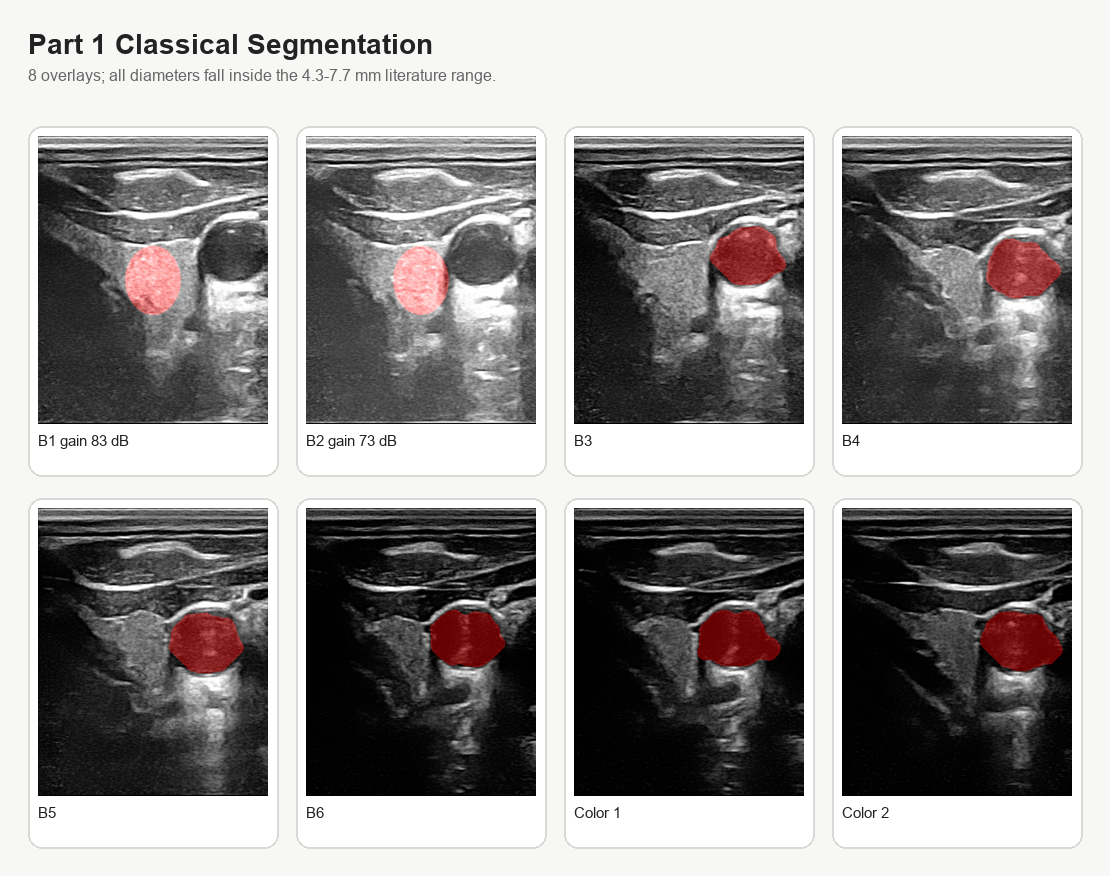
\includegraphics[width=0.98\textwidth]{panel_part1_classical.png}
    \caption{Part 1 classical carotid segmentation overlays for six B-mode and two Color Doppler fallback images.}
    \label{fig:part1_overlay}
\end{figure*}

\begin{figure}[t]
    \centering
    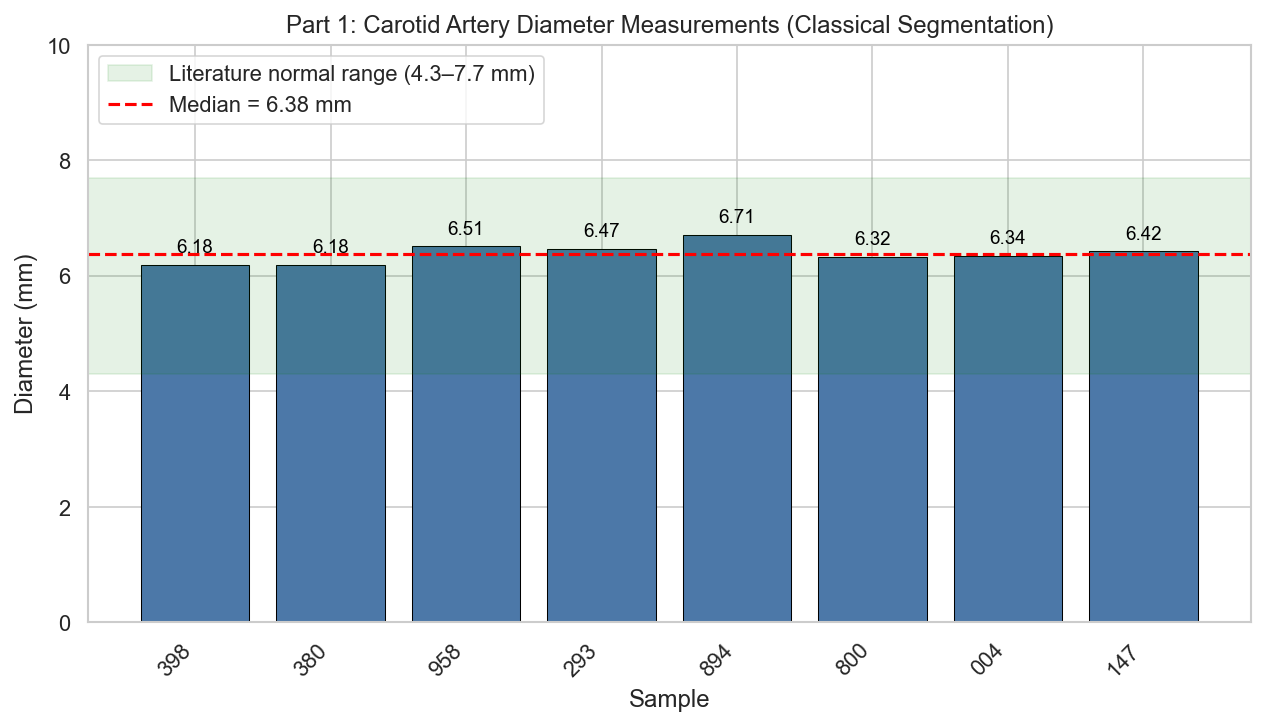
\includegraphics[width=\columnwidth]{fig1a_part1_diameter_summary.png}
    \caption{Carotid artery diameter estimates compared with the literature normal range.}
    \label{fig:part1}
\end{figure}

\subsection{Part 2 Breast Ultrasound Classification}
BUSAT masks achieved the strongest overall classification performance. With SVM, BUSAT reached an accuracy of 0.892 with balanced sensitivity and specificity. With random forest, BUSAT achieved the highest AUC of 0.940. The refined classical segmentation was also competitive, reaching an SVM AUC of 0.924 and random-forest accuracy of 0.875. Table~\ref{tab:part2} summarizes the main results.

\begin{table}[t]
\centering
\caption{Part 2 five-fold cross-validation results.}
\label{tab:part2}
\begin{tabular}{llcc}
\toprule
Mask & Classifier & Accuracy & AUC \\
\midrule
Full & SVM & 0.817 & 0.915 \\
CV & RF & 0.817 & 0.917 \\
Refined & SVM & 0.858 & 0.924 \\
BUSAT & SVM & \textbf{0.892} & 0.937 \\
BUSAT & RF & 0.883 & \textbf{0.940} \\
\bottomrule
\end{tabular}
\end{table}

\begin{figure*}[t]
    \centering
    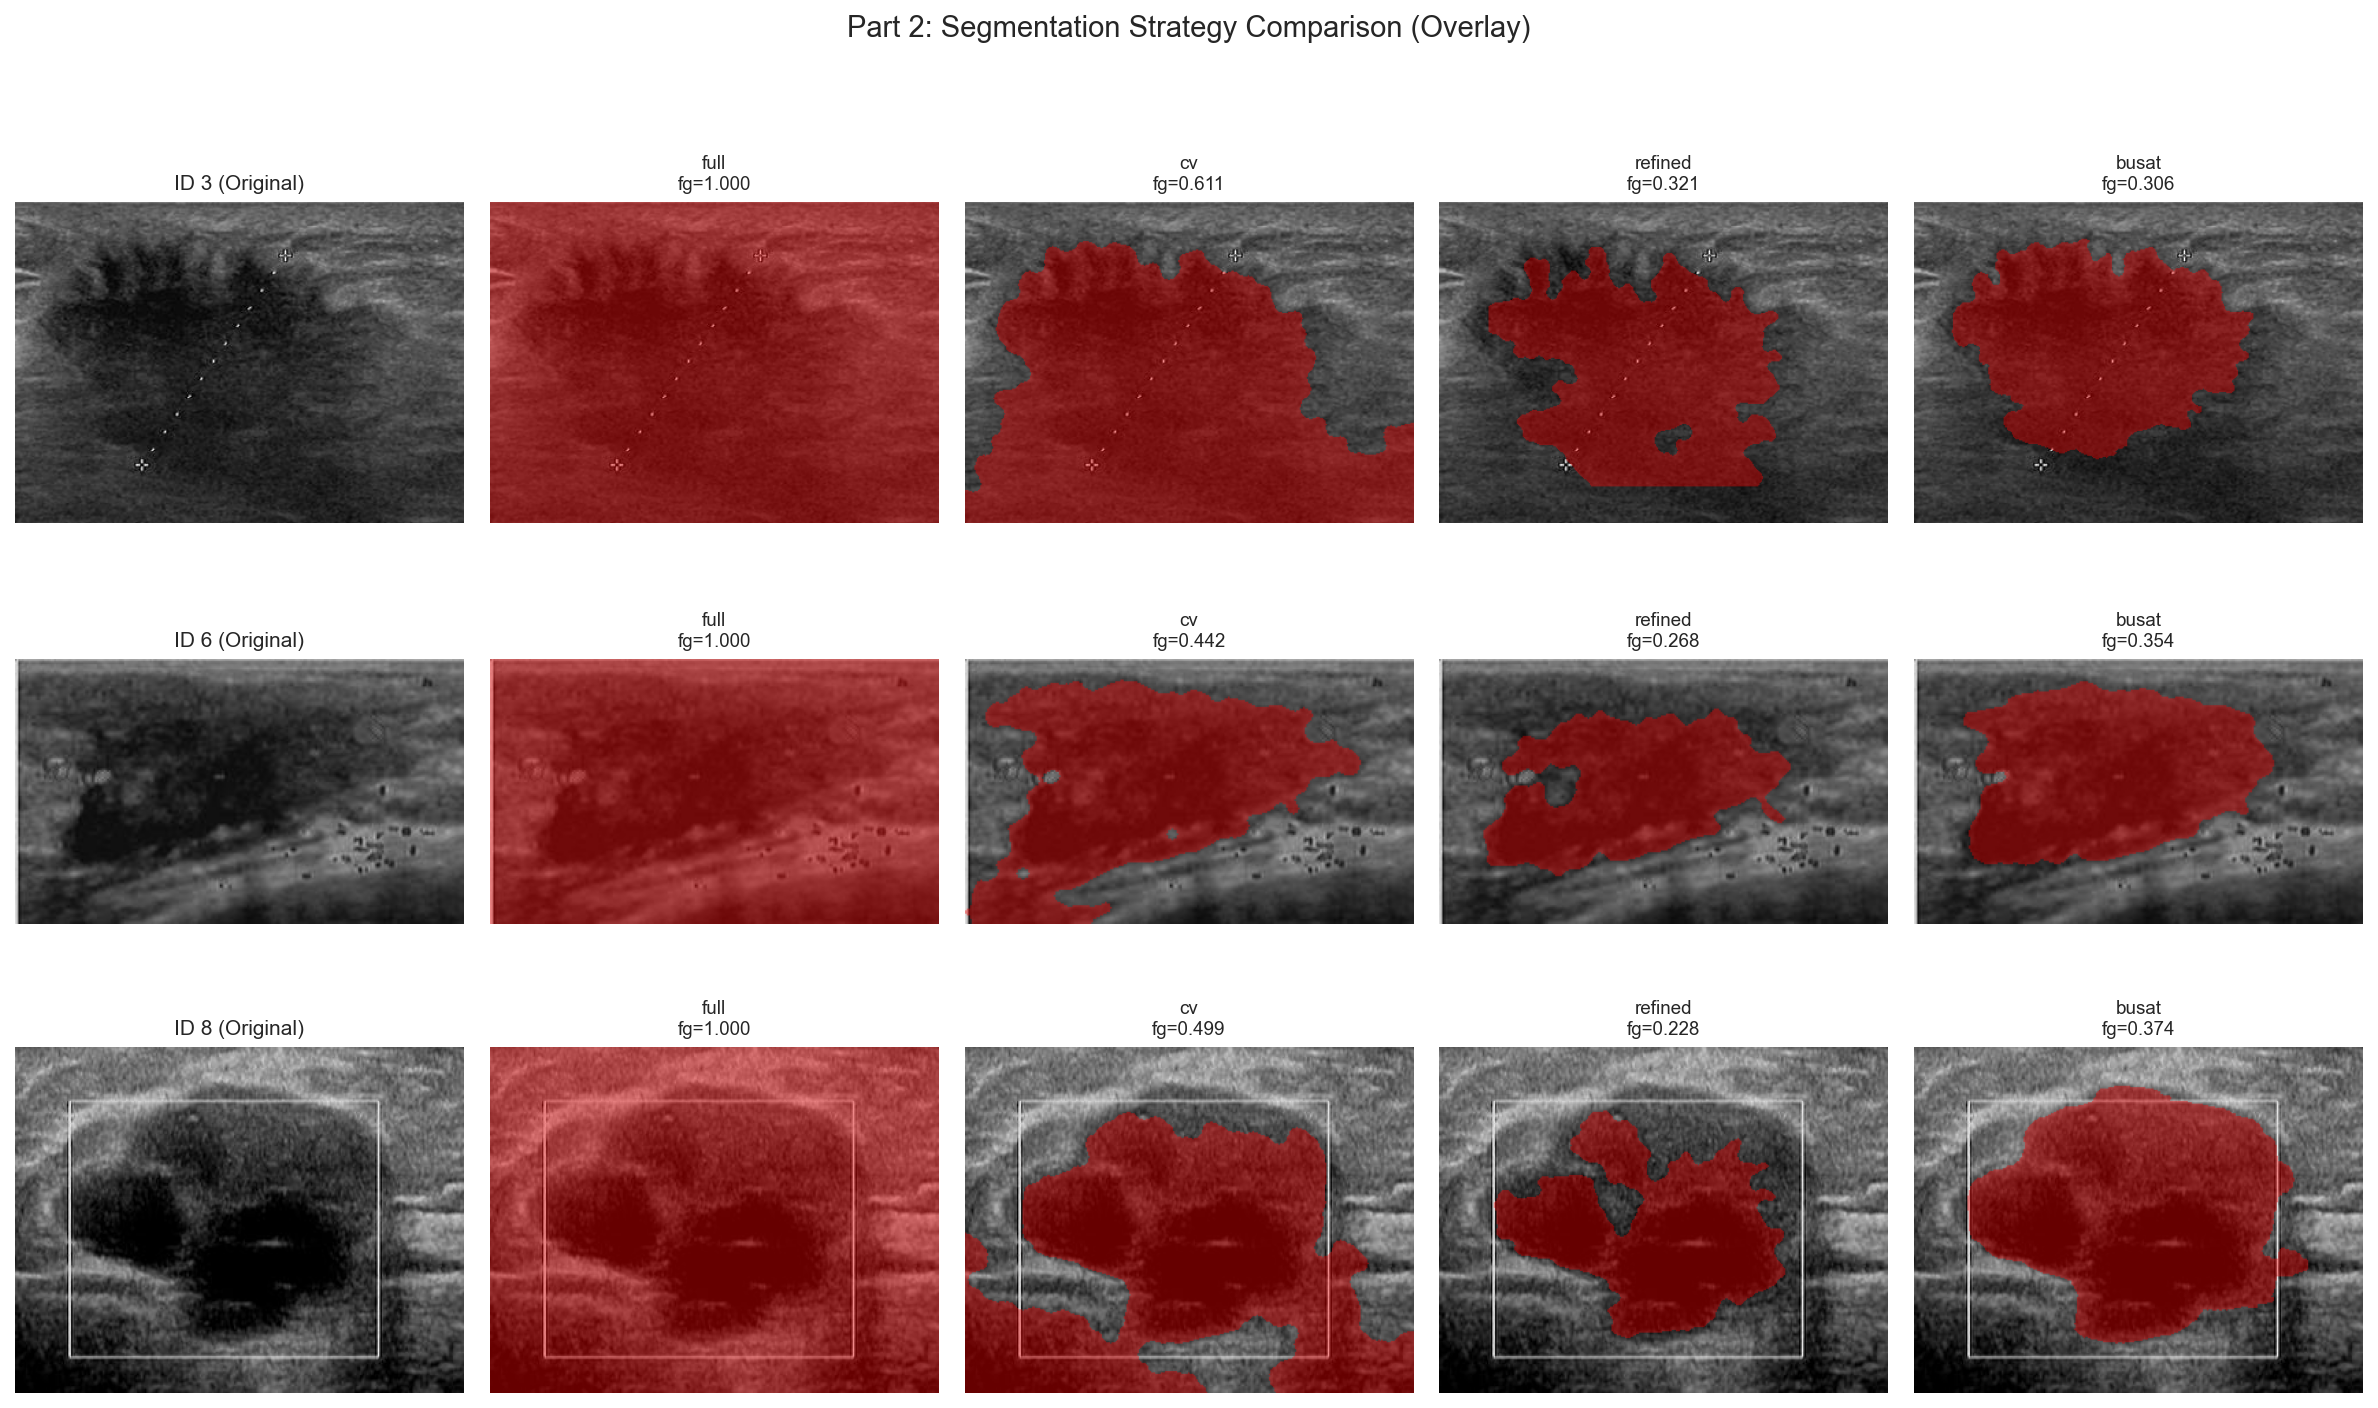
\includegraphics[width=0.98\textwidth]{fig2a_part2_segmentation_examples.png}
    \caption{Visual comparison of Part 2 segmentation strategies. Full-image masks include surrounding tissue, while refined and BUSAT masks better isolate lesion regions.}
    \label{fig:part2_seg}
\end{figure*}

Feature-count analysis showed that classification performance saturated after a moderate number of high-ranked features. This suggests that a small subset of reliable shape and texture features can capture much of the discriminative signal in this dataset. The segmentation-error analysis further showed that using the full image as the mask reduced AUC compared with BUSAT by 0.019--0.060, depending on classifier, confirming that inaccurate masks degrade downstream classification.

\begin{figure*}[t]
    \centering
    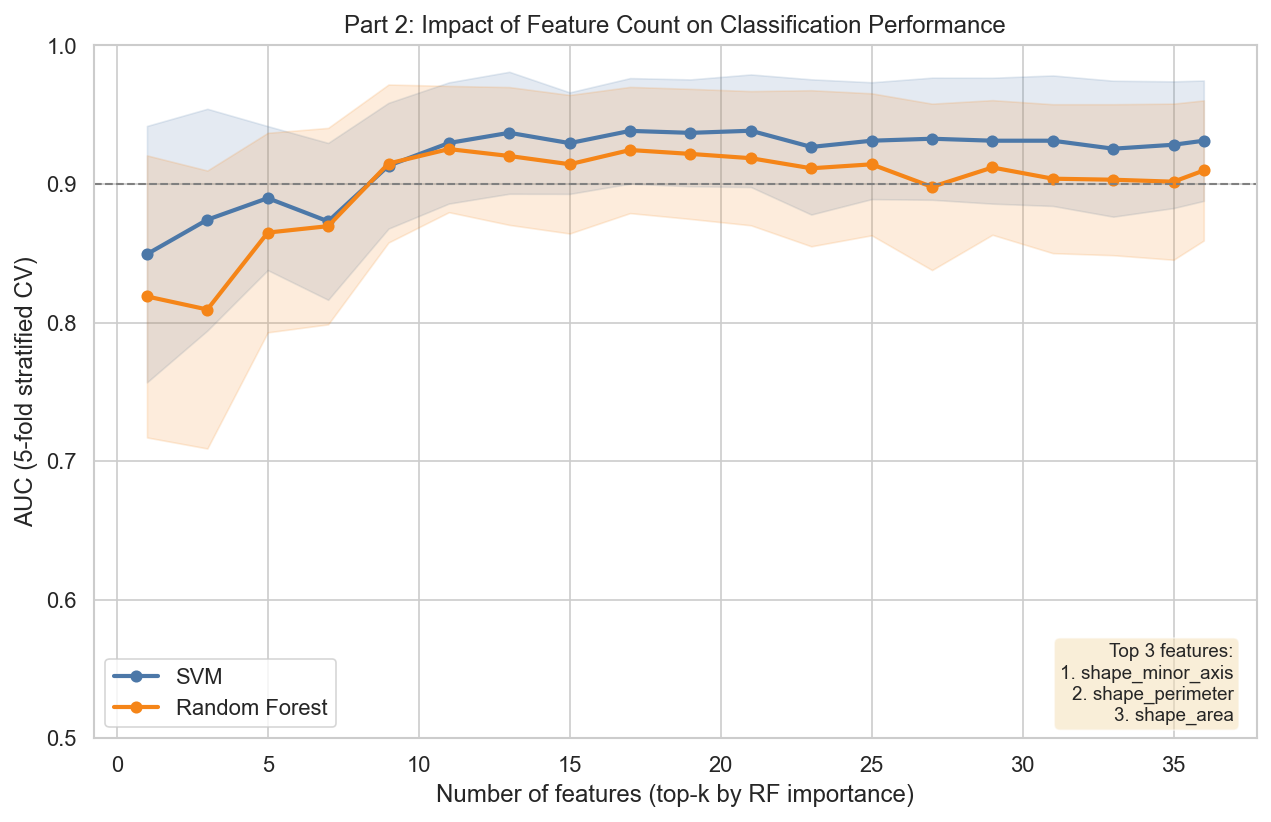
\includegraphics[width=0.49\textwidth]{fig2d_part2_feature_number_impact.png}
    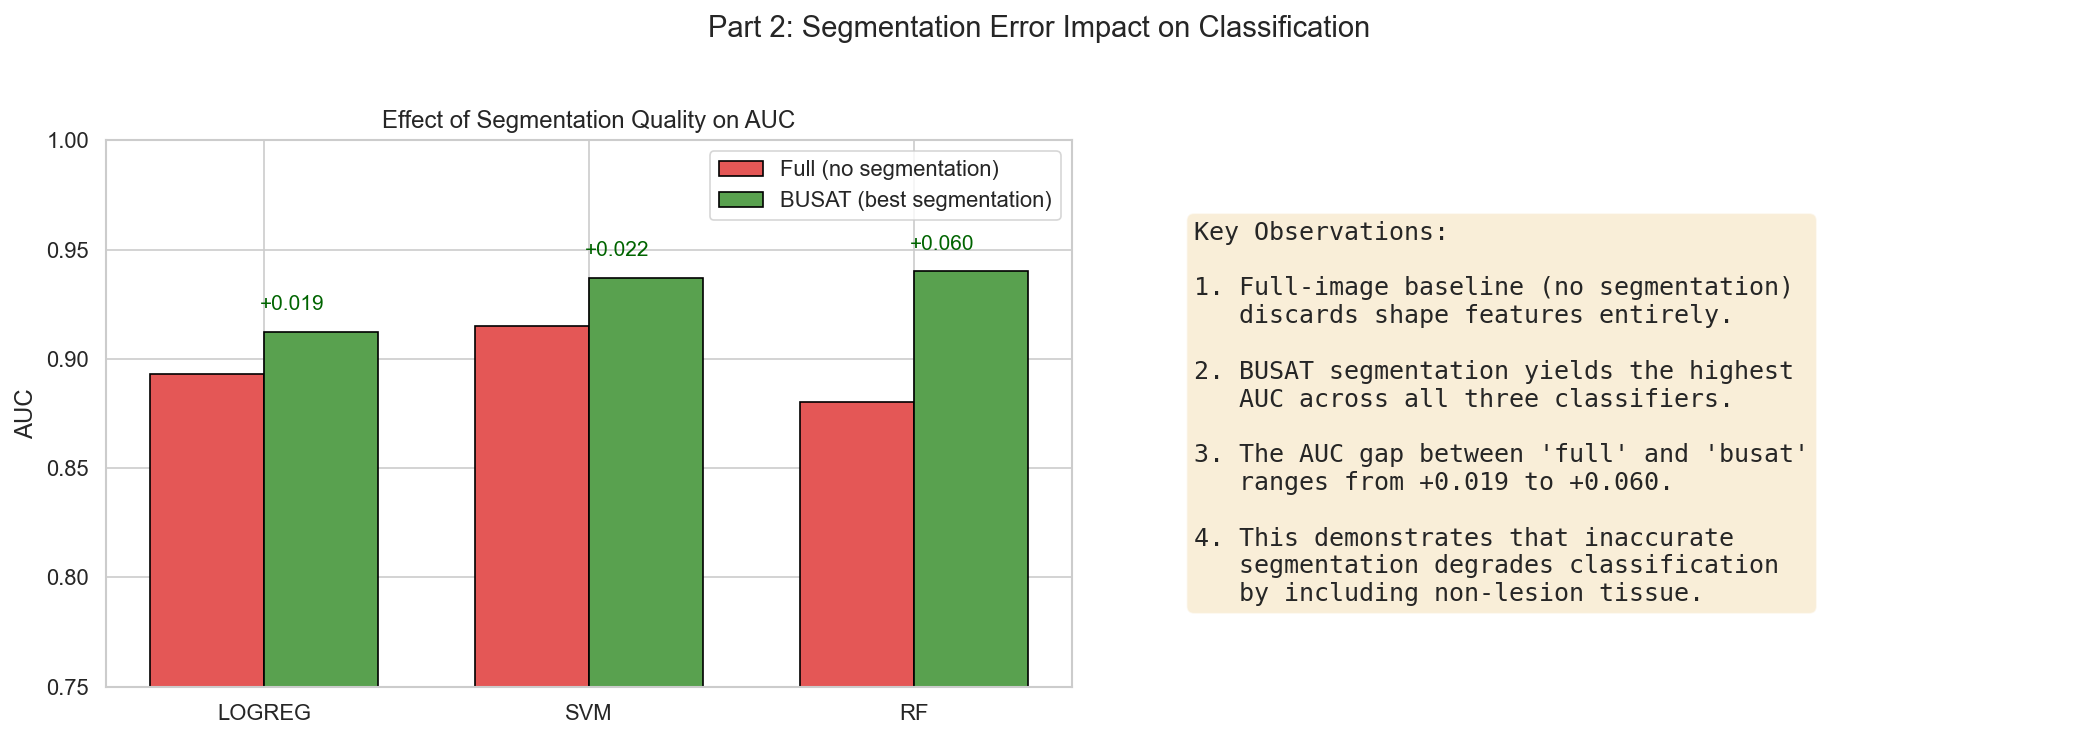
\includegraphics[width=0.49\textwidth]{fig2e_part2_segmentation_error_impact.png}
    \caption{Part 2 ablation studies. Left: feature count impact. Right: segmentation error impact.}
    \label{fig:part2_ablation}
\end{figure*}

\subsection{Part 3 Foundation-Model Analysis}
SAM2 segmentation on Part 1 was strongly prompt-dependent. Six of eight images produced diameters within the literature range, while two crop-center fallback cases failed. On Part 2, SAM2 completed all 120 prompted segmentations with a mean predicted IoU score of 0.680, but visual quality varied across cases.

For classification, BiomedCLIP with SVM achieved the best foundation-model result, with accuracy 0.858 and AUC 0.935. This was close to BUSAT with random forest (AUC 0.940) but did not exceed the best traditional pipeline. Table~\ref{tab:part3} summarizes the comparison.

\begin{table}[t]
\centering
\caption{Part 2 baselines versus Part 3 foundation-model embeddings.}
\label{tab:part3}
\begin{tabular}{llcc}
\toprule
Route & Model & Accuracy & AUC \\
\midrule
BUSAT features & SVM & \textbf{0.892} & 0.937 \\
BUSAT features & RF & 0.883 & \textbf{0.940} \\
OpenCLIP embedding & Logistic & 0.833 & 0.916 \\
BiomedCLIP embedding & SVM & 0.858 & 0.935 \\
BiomedCLIP embedding & RF & 0.850 & 0.928 \\
\bottomrule
\end{tabular}
\end{table}

\begin{figure*}[t]
    \centering
    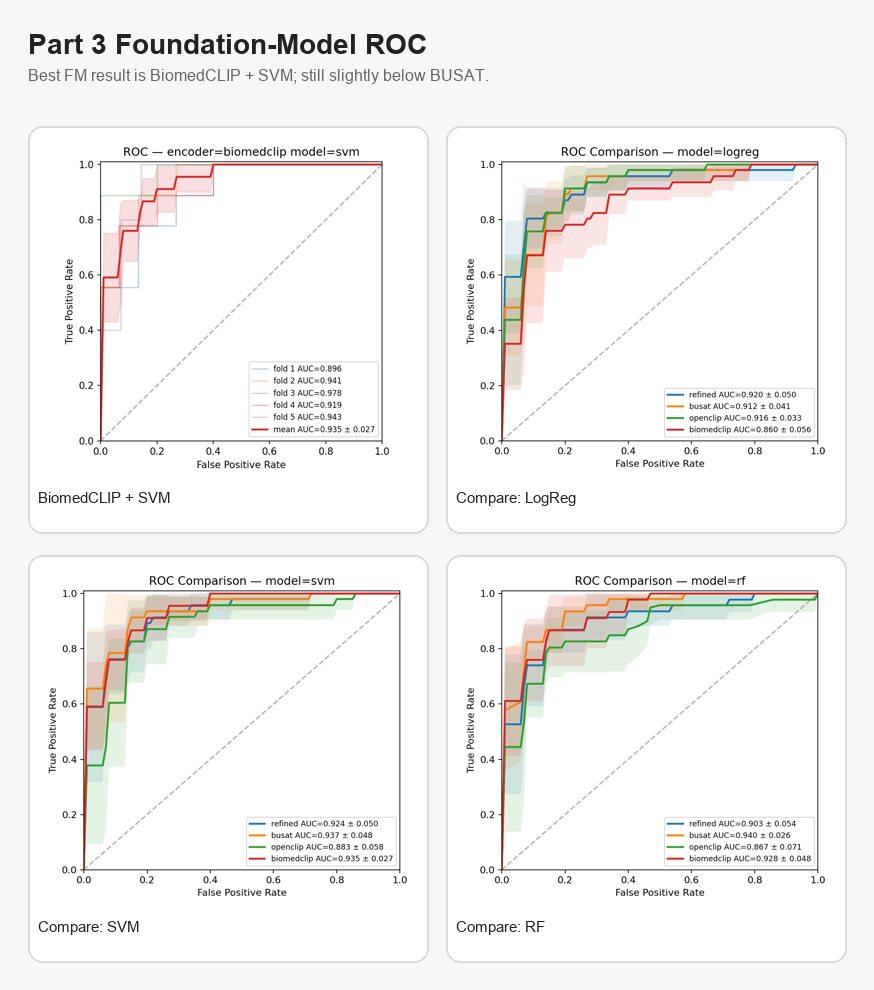
\includegraphics[width=0.98\textwidth]{panel_part3_foundation_roc.png}
    \caption{ROC comparison between foundation-model embeddings and Part 2 baselines. BiomedCLIP approaches but does not surpass the BUSAT baseline.}
    \label{fig:part3_roc}
\end{figure*}

\section{Open Discussion}
\subsection{A Concrete Improvement Idea}
Based on these experiments, a practical improvement direction is an acquisition-aware and uncertainty-driven medical image processing loop. Such a system would not rely on a single model. Instead, it would combine acquisition metadata, image quality control, hybrid segmentation, uncertainty estimation, clinician review, and active learning.

First, ultrasound acquisition parameters should be treated as model inputs. Gain, dynamic range, scan depth, probe frequency, Doppler settings, and pixel spacing directly affect image appearance and measurement reliability. A clinically useful system should use these metadata for normalization, quality assessment, and physical-unit conversion. Second, segmentation should be hybrid. Strong anatomical priors such as Hough candidates can generate prompts for SAM2 or MedSAM \cite{ma2024medsam}, while BUSAT or refined masks can serve as teacher masks for lightweight adaptation on breast ultrasound. Third, uncertainty should be a first-class output. Multi-prompt segmentation, test-time augmentation, calibrated probabilities, and model ensembles can flag cases where small boundary changes alter the final classification or measurement. Finally, clinician corrections should be used for active learning, focusing annotation effort on high-risk and high-uncertainty cases.

\subsection{Future Directions and Concerns}
Medical image processing is likely to move from single-task algorithms toward multimodal, interactive, and regulated clinical assistance systems. Future ultrasound foundation models should learn not only static image texture, but also organ-specific anatomy, video dynamics, device settings, and acquisition quality. They should also output quantitative biomarkers, including lesion size, shape, vascularity, elasticity, and longitudinal change.

However, clinical deployment requires caution. Domain shift across hospitals, probes, operators, and patient populations can degrade model performance. Automation bias may lead clinicians to over-trust confident but incorrect outputs. Standard metrics such as AUC and Dice do not fully capture clinical benefit or harm. Finally, privacy, cybersecurity, model update control, and responsibility assignment must be addressed before continuous-learning systems can be safely deployed. Regulatory frameworks such as FDA guidance on AI-enabled devices and predetermined change control plans are therefore directly relevant \cite{fdaaiml,fdapccp}.

\section{Limitations}
This project has several limitations. The Part 1 acquisition includes only eight images from a healthy subject and does not include manual caliper measurements from the ultrasound device. The Color Doppler acquisitions did not contain reliable color flow and therefore could not validate Doppler-specific segmentation. The Part 2 dataset is small and evaluated with internal cross-validation rather than external multi-center validation. The Part 3 segmentation experiment used a generalist SAM2 checkpoint rather than an ultrasound-specialist segmentation foundation model. Finally, foundation-model classification was evaluated with frozen embeddings and shallow classifiers rather than end-to-end fine-tuning.

\section{Conclusion}
This project implemented and evaluated a complete ultrasound image analysis workflow. Classical carotid segmentation produced physically plausible measurements in Part 1. BUSAT segmentation with shallow classifiers remained the strongest Part 2 breast ultrasound baseline. Foundation-model embeddings, especially BiomedCLIP, approached the BUSAT classification performance without task-specific fine-tuning, but prompted SAM2 segmentation remained sensitive to prompt quality. These results suggest that future medical ultrasound AI systems should combine anatomical priors, acquisition metadata, uncertainty estimation, and clinician feedback rather than relying on a single fully automatic model.

\section*{Acknowledgment}
The authors thank the BME1307 teaching team for providing the project description, ultrasound acquisition guidance, and breast ultrasound sample dataset.

\bibliographystyle{IEEEtran}
\bibliography{references}

\end{document}
